\documentclass{article}
\usepackage[utf8]{inputenc}
\usepackage{multicol}
\usepackage[none]{hyphenat}
\usepackage{amsmath}
\usepackage{amssymb}
\usepackage{listings}
\usepackage{hyperref}

\usepackage{xcolor}

\usepackage[verbose=true,letterpaper]{geometry}
\AtBeginDocument{
  \newgeometry{
    textheight=9in,
    textwidth=6.5in,
    top=1in,
    headheight=14pt,
    headsep=25pt,
    footskip=30pt
  }
}

\definecolor{codegreen}{rgb}{0,0.6,0}
\definecolor{codegray}{rgb}{0.5,0.5,0.5}
\definecolor{codepurple}{rgb}{0.58,0,0.82}
\definecolor{backcolour}{rgb}{0.95,0.95,0.92}

\lstdefinestyle{mystyle}{
    backgroundcolor=\color{backcolour},   
    commentstyle=\color{codegreen},
    keywordstyle=\color{magenta},
    numberstyle=\tiny\color{codegray},
    stringstyle=\color{codepurple},
    basicstyle=\ttfamily\footnotesize,
    breakatwhitespace=false,         
    breaklines=true,                 
    captionpos=b,                    
    keepspaces=true,                 
    numbers=left,                    
    numbersep=5pt,                  
    showspaces=false,                
    showstringspaces=false,
    showtabs=false,                  
    tabsize=2
}

\lstset{style=mystyle}

\usepackage{graphicx}
\graphicspath{ {./images/} }

\title{Guide to Deep Reinforcment Learning for Supply Chain Optimzation}

\author{ {Aditya Chopra} \\
	Consultant (Intern) - CoE Analytics (Data Science) \\
	Happiest Minds Technologies, Bangalore \\
	\texttt{aditya.i.chopra@happiestminds.com} \\
	\texttt{f20190178@hyderabad.bits-pilani.ac.in}
}

\begin{document}

\maketitle

\section{Introduction}

Supply Chain Management is the optimization of resource allocation to an industry, to facilitate efficient production, and maximal profits. We look at the use of Deep Reinforcement Learning Strategies to improve upon existing baseline policies for Supply Chain Management Optimzation. Further, we leverage the use of Deep Neural Networks, to improve the performance of the model.

The code used in this report can be found on: \href{https://github.com/adeecc/SCM-RL}{adeecc/SCM-RL}

% TODO: Add Multicolumns




\section{Components of the Reinforcement Learning Strategy}

\subsection{The Agent and The Environment}
The environment consists of a main Factory, a central factory warehouse, and $W$ distribution warehouses. The environment has the following properties:

A factory produces products with a constant cost of $z_0$ dollars per unit, and the production levela t time $t$ is $a_0(t).$

Further, the facrtory warehouse has a maximum capacity of $c_0$ units. The storage cost for one product unit for one time step at the factory is $z_0^S$, and the stock level at time t is $s_0(t)$.

At any time, $t$, the number of units shipped from the factory warehouse to the distribution warehouse $j$ is $a_j(t)$ and the transportation cost in $z_j^T$ dollars per unit.

Each distribution warehouse $j$ has a maximum capacity of $c_j$, storage cost of $z_j^S$ and stock level at time $t$ equal to $q_j(t)$. Products are sold at a uniform price $p$ and the demand at time $t$ is $d_j(t)$, for the warehouse j. We also assume that the manufacturer is contractually obligated to fulfill all orders placed by retail partners, and if the demand for a certain time step exceeds the corresponding stock level, it results in a penalty of $z_j^P$ dollars per each unfulfilled unit. Unfulfilled demand is carried over between time steps (which corresponds to backordering), and we model it as a negative stock level.

The Demand data being used is from a publicly available demand dataset \cite{zhao_product_2017}. The dataset was preprocessed and the product with maximum entries selected. 

\pagebreak

\subsection{Markov Decision Process}

The problem at hand can be modeled as a Markov Decision Process (represented by a 4-tuple) with a deterministic policy.
\begin{equation}
    \langle S_t, A_t, R_{t+1}, S_{t+1} \rangle
\end{equation}


where, the state at time $t$ is the tuple of all current stock levels, and demand values of all warehouses for $\tau$ previous steps.
\begin{equation}
    S_t = \langle q_0(t), q_1(t), ..., q_W(t), d(t-1), d(t-2), ..., d(t-\tau) \rangle
\end{equation}

\begin{equation}
    d(t) = \langle d_1(t), ..., d_W(t) \rangle
\end{equation}

Since we assume the current state to include just the previous demand values, it can potentially learn the demand function and embed the same into our model parameters.

The state update rule is specified as follows:

\begin{equation}
    \begin{split}
        S_{t+1} = \langle & \min \{ q_0(t) + a_0 - \sum_{j = 1}^W a_j, c_0 \}, \\
        & \min \{ q_1(t) + a_1(t) - d_1(t), c_1 \}, \\
        & ... \\
        & \min \{ q_W(t) + a_W(t) - d_W(t), c_W \}, \\
        & d(t), \\
        & ... \\
        & d(t - \tau) \rangle
    \end{split}
\end{equation}




\begin{figure}[h]
    \centering
    \includegraphics[width=0.7\textwidth]{RL.png}
    \caption{High level visualization of the algorithm}
\end{figure}

And finally, the action vector consists of production and shipping controls,
\begin{equation}
    A_t = \langle a_0(t), a_1(t) ..., a_W(t) \rangle \label{eq:action_fmt}
\end{equation}

The dererministic Policy Function, \( \pi \) is determined by the Reinforcement Learning Model. \( \pi \) is optmized to maximise returns given by:

\begin{equation}
    R = p\sum_{j = 1}^Wd_j - z_0a_0 - \sum_{j = 0}^W z_j^S \max \{q_j, 0 \} - \sum_{j = 1}^W z_j^Ta_j + \sum_{j = 1}^Wz_j^P \min \{q_j, 0 \}
\end{equation}

\subsection{Model Description}

\paragraph{}

We looked at several candidate examples, with multiple hyperparameters (TODO: Put Table) ranging from Deep Q Learning Models, Policy Gradient Algorithms, and Actor-Critic Algorithms. Deep Q Learning Algorithms use Deep Neural Newtorks to approximate the Q-Value function, which are the probabilities of taking a particular action. These models are designed for Discrete Action Spaces, and become extremely ineffective with a continuous action space as ours. Policy Gradient Algorithms use Deep Neural Networks to approximate the policy function directly and work well with continuous action spaces. However, these models are very naive and can't optimize for a complicated problem. 

Actor-Critic models such as Deep Deterministic Policy Gradient (DDPG) Algorithm \cite{lillicrap_continuous_2019} make use of 2 Separate Networks, the Actor and the Critic. The Actor is a Policy Gradient Model, and the Critic a Q Learning Model. Rather than using raw rewards and returns, the policy is computed based on the learned value function. In effect, the critic judges the performance of the actor and both are optimized based on the rewards. However, the DDPG algorithm suffers due to instability in the form of sensitivity to hyper-parameters and propensity to converge to very poor solutions or even diverge. 

\begin{figure}[h]
    \centering
    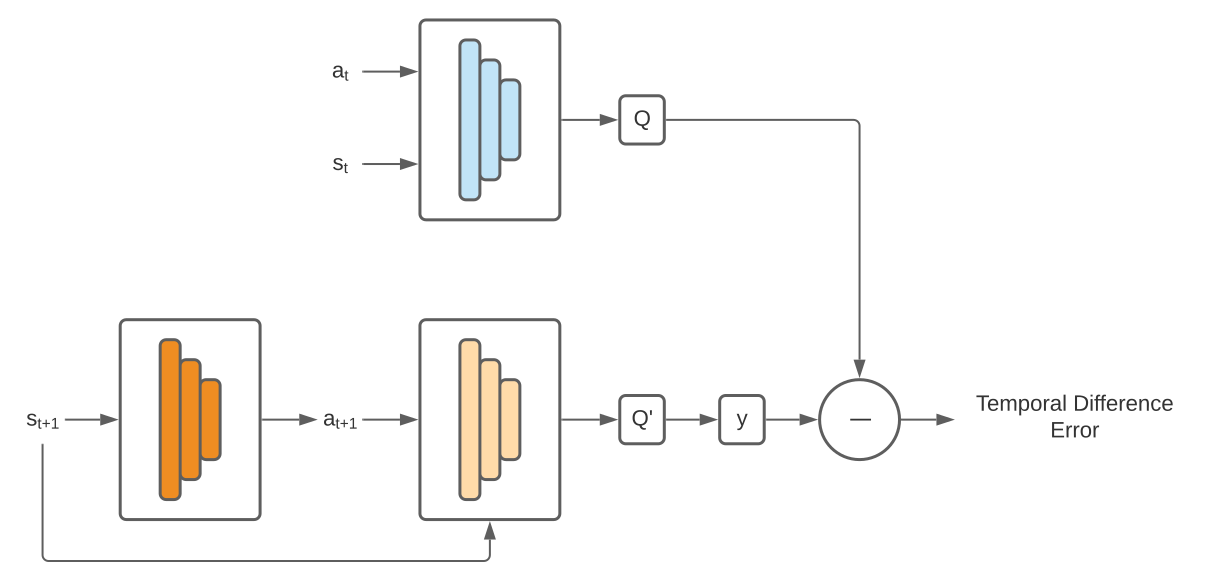
\includegraphics[width=0.9\textwidth]{DDPG.png}
    \caption{Network Architecture of the DDPG Algorithm with Actor and Critic Networks \\ \emph{Note:} TD Error = Temporal Difference Error}
\end{figure}

A common failure mode for DDPG is that the learned Q-function begins to dramatically overestimate Q-values, which then leads to the policy breaking, because it exploits the errors in the Q-function.  Various algorithms have improved stability by addressing well identified issues. One of them is Twin Delayed Deep Deterministic policy gradient (TD3) \cite{fujimoto_addressing_2018}, which uses learns two Q-functions instead of one (hence “twin”), and uses the smaller of the two Q-values to form the targets in the Bellman error loss functions besides other optimizations.

\begin{figure}[h]
    \centering
    \includegraphics[width=0.9\textwidth]{TD3.png}
    \caption{Network Architecture of the TD3 Algorithm with Twin Actor and Critic Networks \\ \emph{Note:} TD Error = Temporal Difference Error}
\end{figure}

As mentioned before, we find are finding a policy that maximises the expected return, \(R\) resulting in the Objective Function and optimzation problem:

\begin{equation}
    \mathcal{J}(\pi_{\theta}) = \mathbb{E}_{S, A, R \sim \pi_{\theta}} \left[ R \right] \end{equation}

\begin{equation}
    \max_{\theta}\mathcal{J}(\pi_{\theta})
\end{equation}





\pagebreak

\section{Training the Model}
\subsection{Creating the OpenAI gym Wrapper}

We create an openAI gym wrapper by inheriting from the \lstinline{ gym.Env} class and implementing the constructor (\lstinline{ __init__}) method, \lstinline{ reset} method and the \lstinline{ step} method.

\begin{lstlisting}[language=Python]
class SimpleSupplyChain(gym.Env):
    def __init__(self, config):
        self.reset()
        self.action_space = Box(low=0.0, high=20.0)
        self.observation_space = Box(low=-10000, high=10000)

    def reset(self):
        self.supply_chain = SupplyChainEnvironment()
        self.state = self.supply_chain.initial_state()
        return self.state.to_array()

    def step(self, action):
        action_obj = Action(self.supply_chain.warehouse_num)
        action_obj.production_level = action[0]
        action_obj.shippings_to_warehouses = action[1:]
        self.state, reward, done = self.supply_chain.step(
            self.state, action_obj)
        return self.state.to_array(), reward, done, {}
\end{lstlisting}

Finally, we use the RLlib package to create a simple model with any desired configuration of Actor Hidden Layers, Critic Hidden Layers, the Discounting Constant \( \gamma \), and other hyperparameters. The setup we used is as follows:

\begin{lstlisting}[language=Python]
config = ddpg.DEFAULT_CONFIG.copy()
config["actor_hiddens"] = [512, 512] 
config["critic_hiddens"] = [512, 512]
config["gamma"] = 0.95
config["timesteps_per_iteration"] = 1000
config["target_network_update_freq"] = 5
config["buffer_size"] = 10000
    
trainer = ddpg.DDPGTrainer(config=config, env=SimpleSupplyChain)
for i in range(n_iterations):
   result = trainer.train()
   print(pretty_print(result))
  
#> Achieved profit: 9238.2
\end{lstlisting}

\subsection{Results}
We ran the model with different parameters and hidden layers. A similar random search based on heuristics can be considered for any other usecase. We compared our model to a baseline (s, Q)-policy which gave mean returns of $6871.0$ in our experimentation. Our model with $(512, 512)$ actor hidden layers and $(512, 512)$ critic hidden layers, gave a mean return of $9238.57$, which is an increase of approximately $34 \%$.


\subsection{Inference from the Model}
The parameters of the model are saved in a json file after trinaing is completed and the same can be loaded. This model needs a state array that can be generated with the available data. This state array can be passed to the \lstinline{policy.compute_single_action} method that returns a vector of actions that need to be taken in the format specified in equation \eqref{eq:action_fmt}.

This same method can be used to generate a graph based visualization of the available stocks in the warehouse, and shipments and hence calculate the profits and cumulative profits.

\subsection{Challenges to overcome}
\subsubsection{Starting the Tensorboard Dashboard}
The model tends to be large, and training it slow even on a dedicated GPU. Training on Google Colab is the sanest option for most people. While on a location machine Tensorboard is the default choice for keeping track of training progress, setting it up on Google Colab is slightly tricky at first, but easy if executed properly.


Load the Tensorboard extension provided by Colab using \lstinline{%load_ext tensorboard}. This loads the \lstinline{tensorboard} magics that can be used to open a local tensorboard instance in the Google Colab window itself.

Use \lstinline{tensorboard --logdir ~/ray_results} to point the directory to where RLlib maintains logs. Start training as you would normally, using the train method provided by RLlib itself.

\subsection{Loading Checkpoints and Trained Models}
RLlib stores the model config as a pickled file and as a json giving the flexibility to use either. However, when the file is stored as a json, the callback functions get stored as a string, rendering the model config unusable. A hack, around this is to set the callbacks manually to the default callbacks proivided by the RLlib library.

The better alternative, is to load the config dictionary from the pickled file using \lstinline{ray.cloudpickle}. The pickled file has the callback functions stored as python methods and is hence easier to use. This is also used in their own linrary in \lstinline{rllib/rollout.py} in their codebase.

\bibliographystyle{ieeetr}
\bibliography{references}

\end{document}
